
\documentclass[12pt]{article}

\usepackage{graphicx}
\graphicspath{ {./images/} }

\usepackage{epsfig}
\usepackage{amsmath,amsthm}
\usepackage{listings}


\newtheorem{lemma}{Lemma}
\newtheorem{theorem}{Theorem}


\usepackage{titlesec}
\titleformat{\section}
{\normalfont\Large\bfseries}{Question~\thesection:}{1em}{}

\newlength{\toppush}
\setlength{\toppush}{2\headheight}
\addtolength{\toppush}{\headsep}


\def\subjnum{Comp 170}
\def\subjname{Computation theory}


\def\doheading#1#2#3{\vfill\eject\vspace*{-\toppush}%
  \vbox{\hbox to\textwidth{{\bf} \subjnum: \subjname \hfil Erli Cai}%
    \hbox to\textwidth{{\bf} Tufts University, Fall 2020 \hfil#3\strut}%
    \hrule}}


\newcommand{\htitle}[1]{\vspace*{1.25ex plus 1ex minus 0ex}%
\begin{center}
{\large\bf #1}
\end{center}} 



\begin{document}
\doheading{2}{title}{Exam}
\setlength\parindent{0pt}


\section{shorties}
a. If A is non-regular, then $ \bar{A}$ is also non-regular\\
Because we know that regular language is closed under complement (if X is regular then $\bar{X}$ is also regular).\\
Then if $\bar{A}$ is regular, then complement of $\bar{A}$, which is just A, will also be regular. This is a contradiction thus $\bar{A}$ is non-regular\\


b. If A and B are Non-regular. $(A \cup B)$ could still be regular.\\
Example: Suppose A is non regular and B = $\bar{A}$. Then B is non-regular (as shown in part a)  and  $(A \cup B) = \Sigma^*$ will be regular.\\

c.  $N = (Q,\Sigma,\Delta,S,F)$ is an NFA and $N' = (Q,\Sigma,\Delta,S,Q\backslash F)$, $L(N') $ is \textbf{not} the complement of $L(N)$\\
Suppose $ s\in \Sigma^*$ and it end up in a set of states $ \{q_1, q_2 | q_1 \in Q \backslash F, q_2 \in Q \}$. Then is accepted by  both N  and $N'$. ($s\in L(N)$ and $s\in L(N')$ ) . $ L(N) \cap L(N') \ne \emptyset$ so they are not complement of each other.\\

d. \\
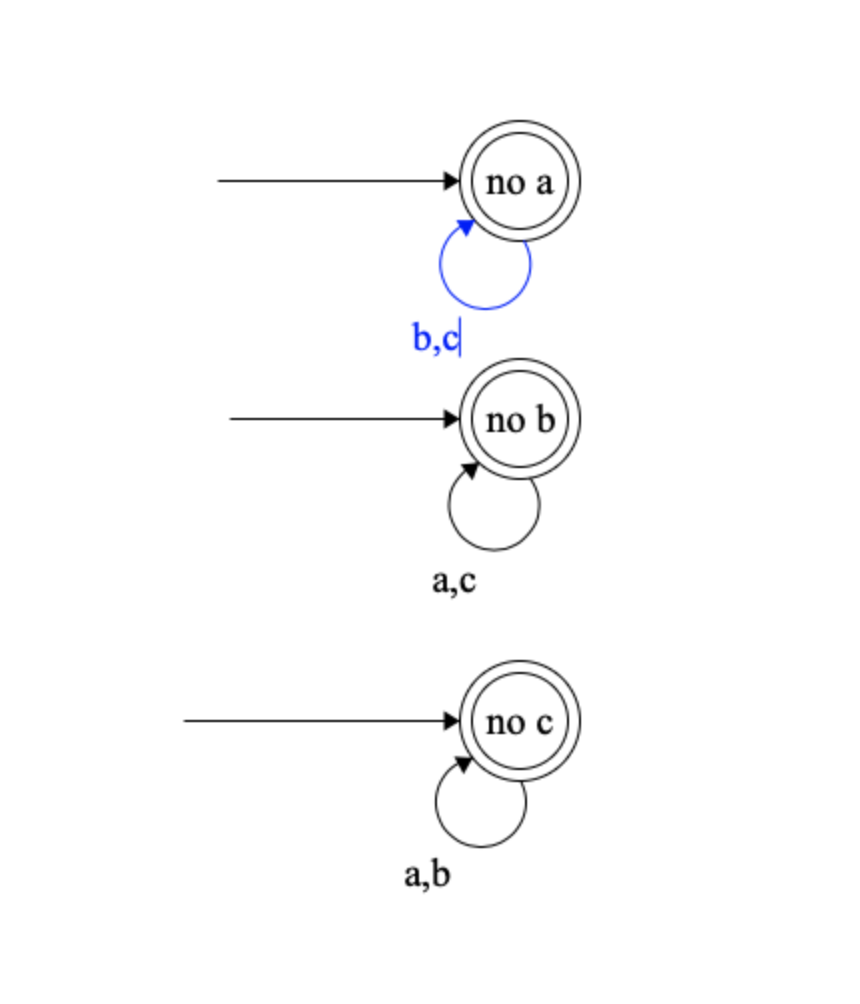
\includegraphics[scale = 0.5]{2}

\pagebreak

\section{Finite Automata}
$mix(A,B) = \{mix(v,w)| v\in A, w\in B, |v| = |w|\}$\\
Suppose A and B are regular languages, then we have\\
$M_A = (Q_A, \Sigma, \delta_A,s_A,F_A)$\\
$M_B = (Q_B, \Sigma, \delta_B,s_B,F_B)$\\
where $L(M_A) = A $ and $L(M_B) = B$\\
To show that mix(A,B) is also regular, we construct a NFA $M = (Q, \Sigma, \delta, s, F)$ such that $L(M) = mix(A,B)$
\begin{flalign*}
Q &= Q_A \times Q_B \times \{1,0\} &&\\
\delta((a,b,0),x) & = (\delta_A(a,x),b,1)\\
\delta((a,b,1),x) & = (a,\delta_B(b,x),1)\\
s &= (s_A,s_B,0)\\
F &= (f_a,f_b,0) \quad\mbox{ for } f_a\in F_A, f_b \in F_B
\end{flalign*}

The state of M is a 3-tuple with the first element  from $Q_A$, second element from $Q_B$ and third element from \{0,1\} indicating whether next character is from A or from B. In each transition, the third element alternate between 0 and 1, and while it equals to 0 we apply transition $Q_A$ to first element , while it equals to 1 we apply transition $ Q_B $ to second element.\\

A string is accepted if first two elements are from Accepted state of A and B respectively. And third element is 0 indicating that the element if of even length.
\pagebreak

\section{Machines to Expressions}
Add a super start state and super accepted state\\
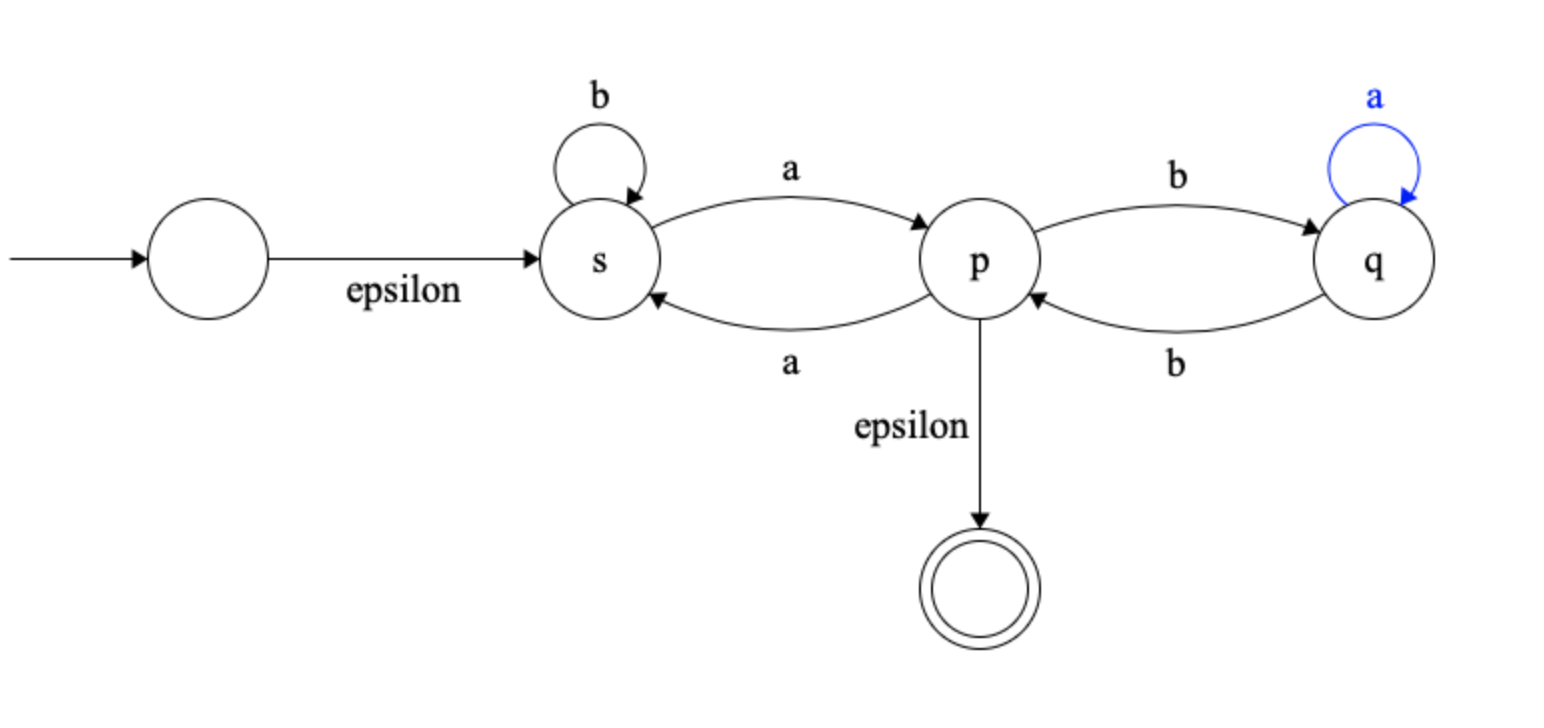
\includegraphics[scale = 0.5]{3}\\
eliminate state q\\
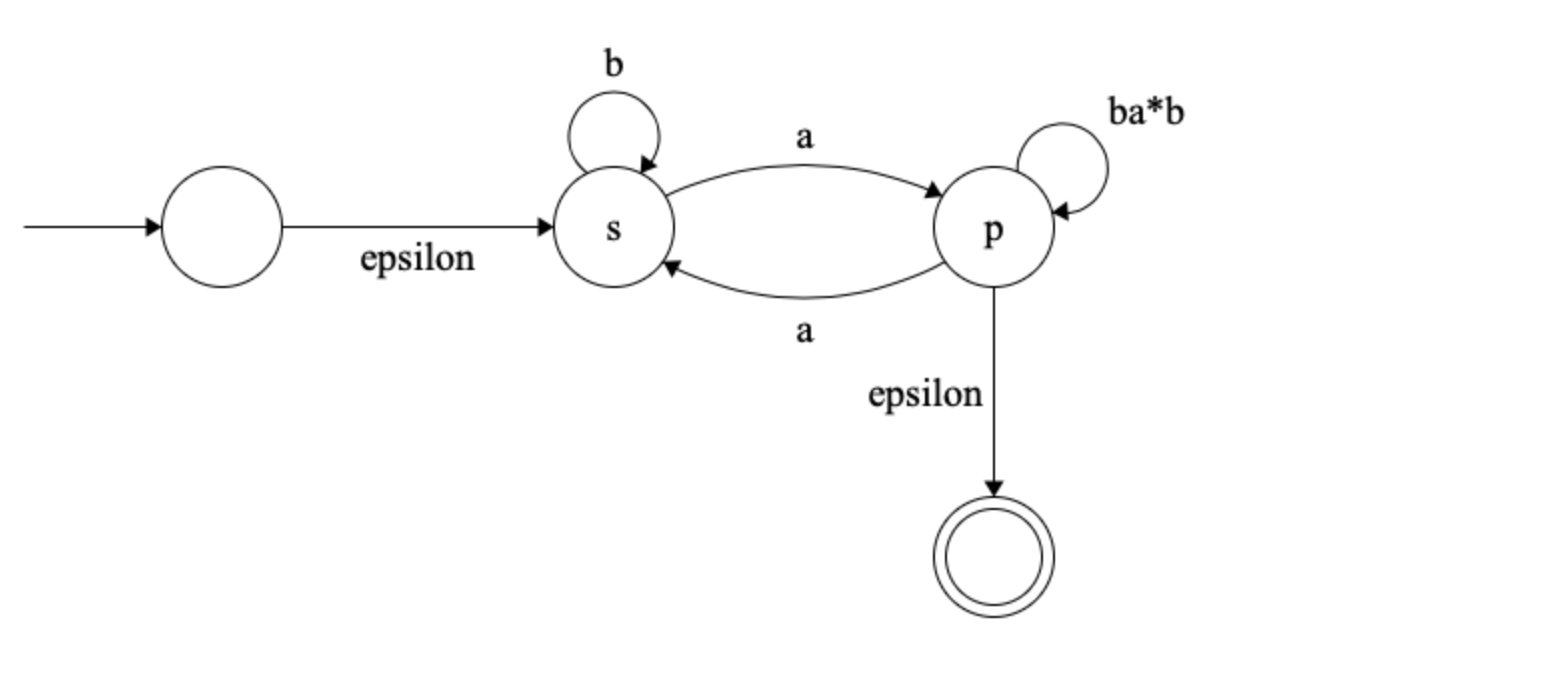
\includegraphics[scale = 0.5]{4}\\
\pagebreak

eliminate state s\\
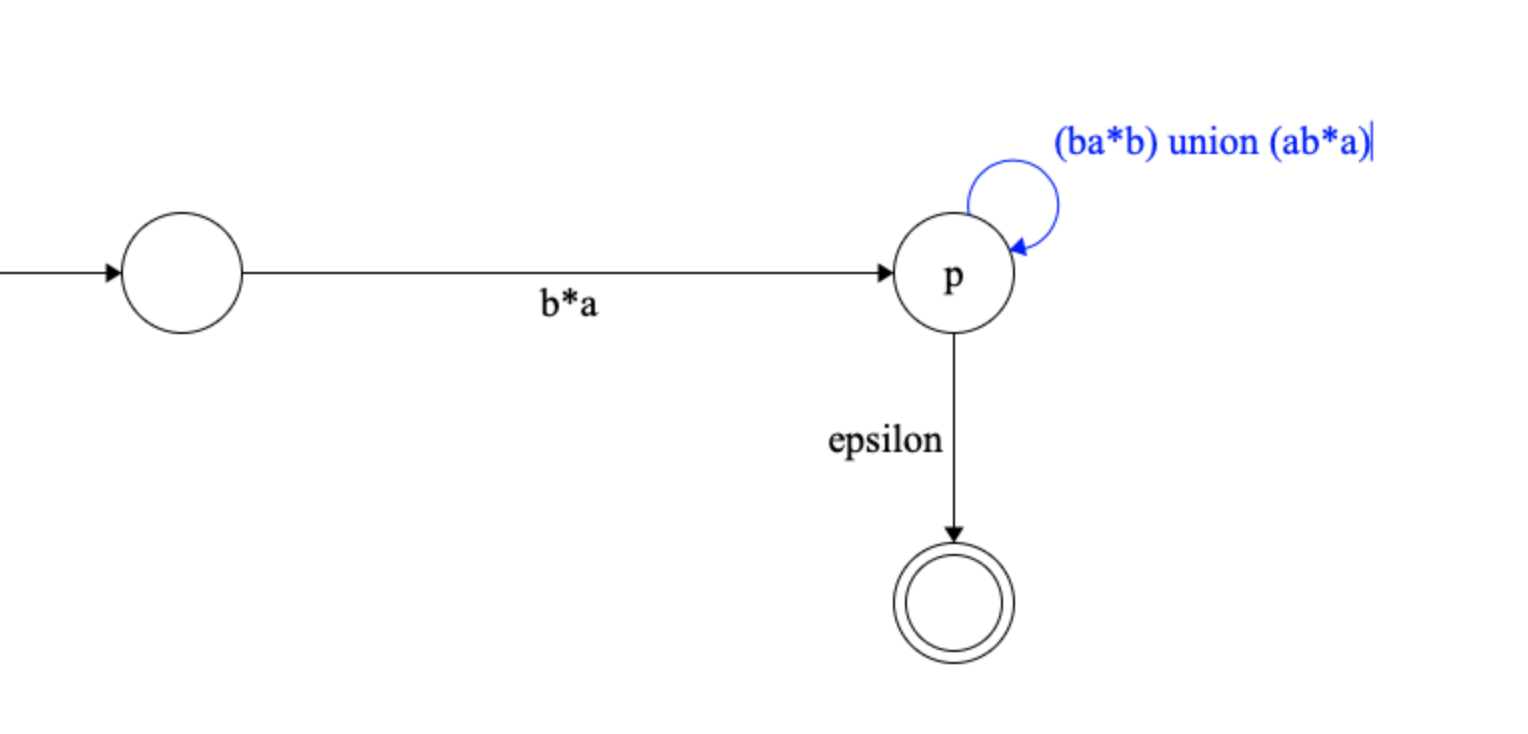
\includegraphics[scale = 0.5]{5}\\
eliminate state p\\
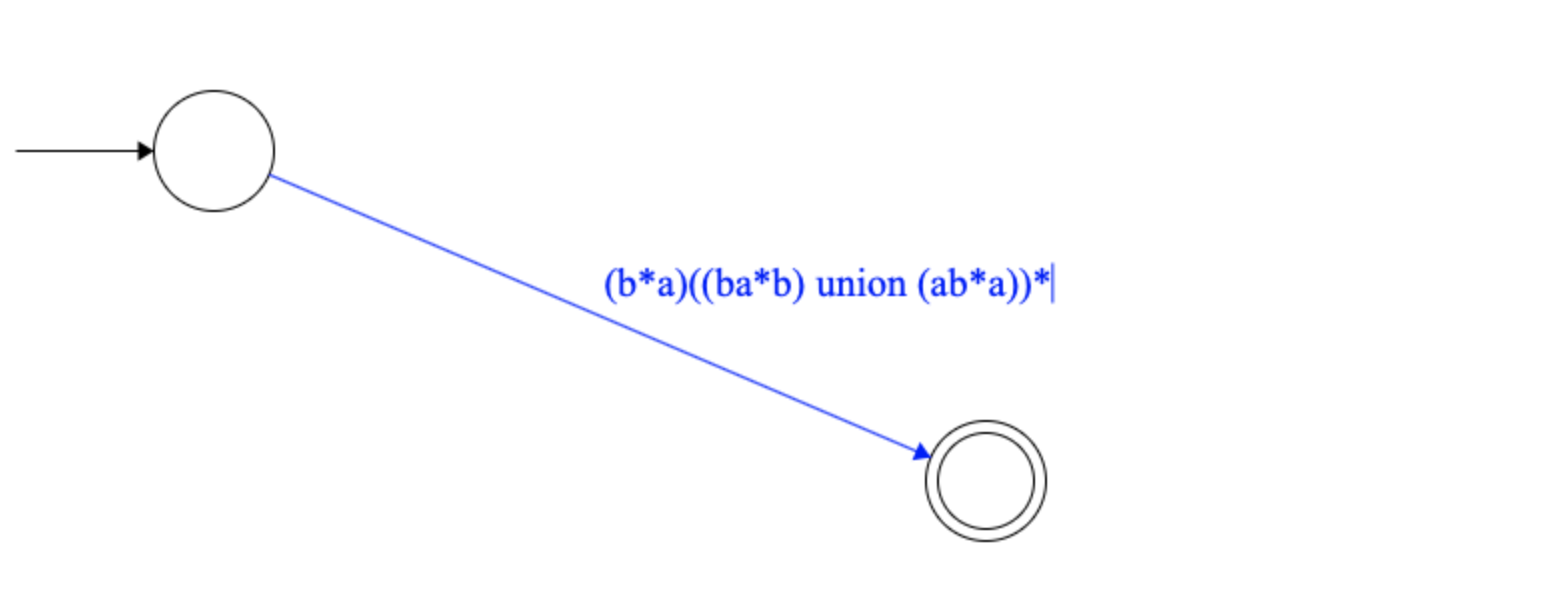
\includegraphics[scale = 0.5]{6}\\
Thus $R = (ba*)((ba*b)\cup (ab*a))*$

\pagebreak


\section{Non-Regular}

Let A be the set of all odd-length strings over \{a, b\} whose middle character is a.
 Assume A is regular: then pumping lemma should be true.\\

For any $p >0$,\\
we pick $w = b^pa a^p $\\
we then write $w = xyz$ where $|y| > 0$ and  $ |xy| <= p$\\
Then y must be a string of b's ($y = b^k$, $ p >= k >1$)\\
If we pump y twice, we have $w' = b^{p+k}aa^p$.\\
If k is odd, then w' is of even length, so it is not in A.\\
If k is even, the middle character of $w'$ should be ($p+\frac{k}{2}+1$)-th element character which must be a b. So it is not in A\\
It contradicts to Pumping Lemma. Thus our assumption that A regular is false. A is non-regular




\pagebreak
\section{CFGs}
$S \rightarrow   aSb|bSa|aAb|bAa$\\
$A \rightarrow   a|b|aa|bb|aAa|bAb|aSa|bSb$\\

Explanation: A non-palindrome string must be asymmetric from center of the string. In my CFG, A will add symmetric part and S will add asymmetric part. Since S can't get to any terminals, we must have a at least one derivation from S to something, which means there will be some asymmetric part in the string and the string is non-palindrome


\end{document}


